\section{The Proposed Model}\label{model}
In this section, we first describe the Decentralized Matrix Factorization (DMF) problem and define notations. 
We then present the basic DMF framework where users individually learn their MF model without communicating with each other. 
Next, we propose a nearby collaborative DMF framework by analysing the data of POI recommendation. 
Then, we present a random walk enhanced nearby collaborative DMF framework. 
Finally, we analysis our model complexity, including communication and computation complexities.

\subsection{Preliminary}

Formally, let $\mathcal{U}$ and $\mathcal{V}$ be the user and item (POI) set with $I$ and $J$ denoting user size and item size, respectively. 
Let $(i,j)$ be an interaction between user $i$ and item $j$, and $r_{ij}$ be the rating of user $i \in \mathcal{U}$ on item $j \in \mathcal{V}$. 
Usually, $r_{ij}$ is a real value in a certain region, and without loss of generality, we assume $r_{ij}$ ranges in [0, 1] in this paper.
Let $\mathcal{O}$ be the training dataset, where all the user-item ratings in it are known. 
%We also use $\mathcal{O}_u$ and $\mathcal{O}_v$ to denote the users and items in the training dataset, respectively. 

For the traditional centralized MF, it first collects all the $r_{ij} \in \mathcal{O}$, and then learns $\textbf{U}\in \mathbb{R}^{K\times{}I}$ and $\textbf{V}\in \mathbb{R}^{K\times{}J}$ using MF technique (Equation \ref{lfm}). 
Here, $\textbf{U}\in \mathbb{R}^{K\times{}I}$ and $\textbf{V}\in \mathbb{R}^{K\times{}J}$ denote the user and item latent factor matrices, with their column vectors $u_i$ and $v_j$ be the $K$-dimensional latent factors for user $i$ and item $j$, respectively.

For DMF, all the known ratings are saved on each user's hand, and consequently, the MF model needs also to be trained on each user's hand to make sure privacy. 
To do this, we use $\textbf{U}\in \mathbb{R}^{K\times{}I}$ to denote user latent factor matrix, with each column vector $u_i$ denotes the $K$-dimensional latent factors for user $i$. 
We also use $\textbf{V}\in \mathbb{R}^{I\times{}K\times{}J}$ to denote item latent factor tensor, with $\textbf{V}^i\in \mathbb{R}^{K\times{}J}$ denotes the item latent factor matrix for user $i$, and further with $v^i_j$ denotes the $K$-dimensional latent factors for item $j$ of user $i$. 
Thus, each user $i$ only need to store his own $K$-dimensional latent factor $u_i$, and an item latent factor matrix $\textbf{V}^i$.

Besides, users need to collaboratively learn their stored factors, i.e., $u_i$ and $\textbf{V}^i$, in decentralized MF scenario. 
For centralized MF, all the users share the same item latent factor matrix, i.e., $\textbf{V}^i=\textbf{V}^{i'}, \forall ~ i,i' \in \mathcal{U}$. %for any two user $i$ and $i'$. 
%all the ratings of $r_{ij} \in \mathcal{O}$ will affect $\textbf{V}$ during training. 
For DMF, each user stores his $u_i$ and $\textbf{V}^i$, and they should be trained collaboratively with other users---which we call `neighbors'. 
Suppose we have a user adjacent graph $\mathcal{G}$, we use $\textbf{W}\in \mathbb{R}^{I\times{}I}$ to denote user adjacency matrix, where each element $w_{i,i'} \subset [0, 1]$ denotes relationship degree between user $i$ and $i'$. Of course, user $i$ and $i'$ have no relationship if $w_{i,i'}=0$. 
We generally use $\mathcal{N}(i)$ to denote the direct neighbors of $i$ on $\mathcal{G}$, $\mathcal{N}^d(i)$ to denote the $d^{st}$ order neighbors of $i$ on $\mathcal{G}$, and $|\mathcal{N}^D(i)|$ as the size the $d^{st}$ order neighbors where $d \in \{1,2,...,D\}$. 
Obviously, $\mathcal{N}^1(i)$ denotes the direct neighbors of $i$, i.e., $\mathcal{N}^1(i)=\mathcal{N}(i)$. 
Besides, to save communication cost, we use $N$ to denote the maximum number of direct neighbors of each user. 
%we use $\textbf{E}\in \{0,1\}^{I\times{}I}$ to denote the adjacency matrix, where each element $e_{i,i'} \in \{0,1\}$ denotes absence of edge between user $i$ and $i'$ or not. 
%We also use $\textbf{W}\in \mathbb{R}^{I\times{}I}$ to denote the relationship degree matrix, where each element $w_{i,i'} \subset [-1, 1]$ denotes relationship degree between user $i$ and $i'$.

Decentralized MF aims to learn $u_i$ and $\textbf{V}^i$ for each user, the model learning procedure are performed on his/her own hand, e.g., Cellphone and Pad.

\subsection{The Basic DMF Framework}
The same as the centralized MF, DMF aims to minimize loss for all the users. 
For each user $i$, the loss funcion is $f(u_i,V^i)=l(r,u_i,V^i)$, where $l(r,u_i,V^i)$ can be least square loss
\begin{equation}
l(r,u_i,V^i)=\frac{1}{2}\sum\limits_{j=1}^{J}{\left(r_{ij} - u_i^T v^i_j\right)}^2,
\end{equation} 
which tries to minimize the error between real ratings and predited ratings \cite{mnih2007probabilistic}, 
or listwise loss 
% \begin{equation}\small
% l(r,u_i,V)=-\sum\limits_{j=1}^{J}{I_{ij}\frac{exp(r_{ij})}{\sum\limits_{k=1}^{J}{I_{ik}exp{(r_{ik})}}}}{log\frac{exp(u_i^T v^i_j)}{\sum\limits_{k=1}^{J}{I_{ik}exp{(u_i^T v_j)}}}},
% \end{equation} 
% which reflects the uncertainty between the training lists and the output lists 
\cite{shi2010list}
% One can use pairwise loss as well
and pairwise loss \cite{rendle2009bpr}. 
In this paper, we will take least square loss as an example. 
Suppose users under the basic DMF framework do not communicate with each other, that is, each user train a MF model only using their own data, without collaborative with each other. 
Then, the corresponding optimization problem of the basic DMF using least square loss for all the users is
\begin{equation}\label{basicdmf}
\mathop { \min }\limits_{u_i,v^i_j \in \mathbb{R}^K} \mathcal{L} = \sum\limits_{i=1}^{I} l(r,u_i,v^i) + \frac{\lambda}{2} \sum\limits_{i=1}^I \left( ||{u_i}||_F^2 + \sum\limits_{j=1}^J||v^i_j||_F^2 \right),
\end{equation} 
where the second regularization term is used to avoid overfitting. 

\subsection{Nearby Collaborative DMF Framework}
The essence of MF is that the user and item latent factors are learnt collaboratively, so should be DMF. 
Thus, \textit{how to collaboratively learn user and item latent factors under DMF framework} becomes a challenging question. 
We answer this question by first analysis the data in POI recommendation scenarios. 

% Most of these loss function can be optimized by using stochastic gradient-descent. 
% Take least square loss for example, for each observed rating $r_{ij} \in \mathcal{O}$, the gradients with respect to $u_i$ and $v^i_j$ are:
% \begin{equation}
% \label{usergradient}
% \frac{\partial \mathcal{L}}{\partial u_i} = -{\left(r_{ij} - u_i^T v^i_j\right)}v^i_j + \lambda u_{i},
% \end{equation} 
% \begin{equation}
% \label{itemgradient}
% \frac{\partial \mathcal{L}}{\partial v^i_j} = -{\left(r_{ij} - u_i^T v^i_j\right)}u_i + \lambda v^i_j.
% \end{equation} 


\textbf{Observation.} 
The user adjacent graph can be built using whatever information that is available, e.g., rating similarity \cite{su2009survey} and user social relationship \cite{yang2011like}. 
However, in DMF for POI recommendation scenario, users' rating are in their own hand, and social relationship is not always available. 
Thus, we focus on using user geographical information to build user adjacent graph, similar as the existing researches \cite{ye2011exploiting,cho2011friendship,cheng2012fused}. 
%The key of optimizing DMF is how to collaborate users for updating latent factors, that is how to select collaborative users. 
%, meanwhile preserve user privacy. 
%Existing researches have shown that POI data follows power law distribution \cite{ye2011exploiting} and Gaussian distribution \cite{cho2011friendship,cheng2012fused}. 
%Inspired by the existing researches \cite{ye2011exploiting,cho2011friendship,cheng2012fused}, we find a simple way to this by data analysis. 
We do this by first analysis the data in POI recommendation scenarios. 
Figure \ref{dataanalysis} shows the rating distributions on two real datasets, i.e., \emph{Foursquare} and \emph{Alipay}. 
Both datasets contain user-item-action-location records, and we simply divide locations into different cities, which we will further describe in details later in experiments. 
We randomly select the user-item-action records in five cities, and plot their rating distributions in Figure \ref{dataanalysis}, where each dot denotes a user-item-action record. 
From it, we have the following observation: 
in POI scenarios, most users only active in a certain city, and we call it ``location aggregation''. 
Only a few users active in multi-cities, which is neglectable. 

% \begin{figure}[!tp]
% \centering
% 
\includegraphics[width=4cm]{figures/graph}
% %\vskip -0.1in
% \caption{User Adjacent Graph.}
% \label{graph}
% %\vskip -0.15in
% \end{figure}

\textbf{User Adjacent Graph. }
The user adjacency graph represents the communication among users. 
%As we analysised, users in POI scenarios tend to have ``location aggregation'' property. 
We build user adjacent graph based on their geographical information. 
Specifically, suppose %$(x^i, x^i)$ and $(x^{i'}, y^{i'})$ are the current latitude and longitude of user $i$ and $i'$ respectively, 
$d_{i,i'}$ is the distance between user $i$ and $i'$, 
the relationship degree between $i$ and $i'$ is 
\begin{equation}
%w_{i,i'} = I^{i,i'} \cdot f((x^i, x^i),(x^{i'}, y^{i'})),
w_{i,i'} = I^{i,i'} \Large \cdot f(d_{i,i'}),
%w_{i,i'}=
%\begin{cases}
%0 & \text{if $i$ and $i'$ in the same city}\\
%f((x^i, x^i),(x^{i'}, y^{i'}))& \text{else}
%\end{cases}
\end{equation} 
where $w_{i,i'} \in [0,1]$, $I^{i,i'}$ is the indicator function that equals to 1 if $i$ and $i'$ are in the same city and 0 otherwise, and $f(d_{i,i'})$ is a mapping function of distance and relationship degree, and the smaller the distance of $i$ and $i'$ is, the bigger their relationship degree is. 
Existing reesarch has proposed different such mapping funciton \cite{zhao2016survey}, which is not our focus. 
Moreover, the number of neighbors determinte the communication cost, and thus, in practice, the communication should only be done in a certain number of users. 
We use $N$ to denote the maximum number of neighbors of user adjacent graph, and these neighbor are chosen based on their geographical distance. 

\begin{algorithm*}[t]
\caption{Nearby Collaborative DMF Optimization Framework}\label{dmflearning}
\KwIn {training ratings ($\mathcal{O}$), learning rate ($\alpha$), user adjacency matrix ($W$), regularization strength($\lambda$), and maximum iterations ($T$)}
\KwOut{user latent factor matrix $\textbf{U}$, and item latent factor tensor $\textbf{V}$}
\For{$i=1$ to $I$}{
	Initialize $u_i$ and $V^i$
}
\For{$t=1$ to $T$}
{
	Shuffle training data $\mathcal{O}$\\
	\For{$r_{ij}$ in $\mathcal{O}$}{
		Calculate $\frac{\partial \mathcal{L}}{\partial u_i}$ and $\frac{\partial \mathcal{L}}{\partial v^i_j}$ based on Equation \ref{usergradient} and Equation \ref{itemgradient}\\
		% Calculate $\frac{\partial \mathcal{L}}{\partial v^i_j}$ based on Equation \ref{itemgradient}\\
		Update $u_i$ and $v^i_j$ by $u_i \leftarrow u_i - \alpha\frac{\partial \mathcal{L}}{\partial u_i}$, $v^i_j \leftarrow v^i_j - \alpha\frac{\partial \mathcal{L}}{\partial v^i_j}$\\
		% Update $v^i_j$ by $v^i_j \leftarrow v^i_j - \alpha\frac{\partial \mathcal{L}}{\partial v^i_j}$\\
		User communication and item latent tensor update (in Algorithm \ref{dmfdirectneighbor} and its enhanced version in Algorithm \ref{dmfrandomwalk})
	}
}
\Return $\textbf{U}$ and $\textbf{V}$
\end{algorithm*}


\begin{figure}
\centering
\subfigure[Foursquare dataset] { 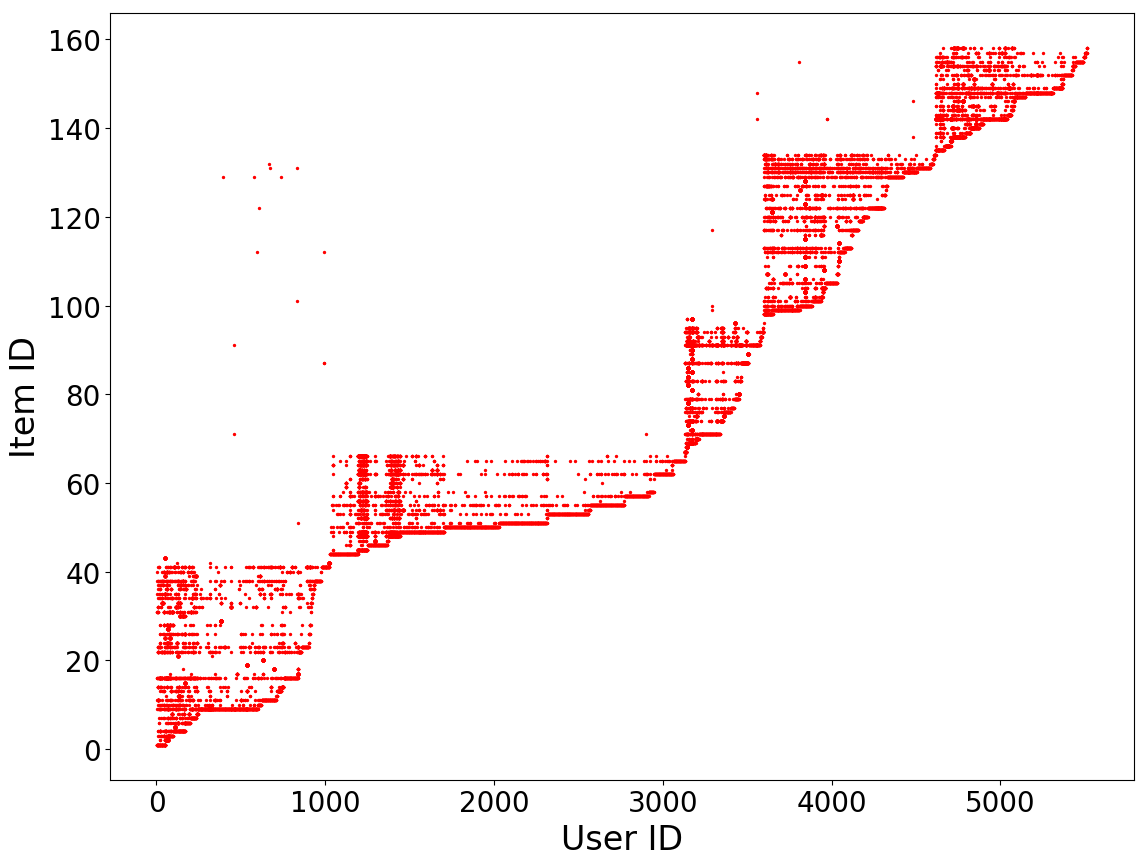
\includegraphics[width=4cm,height=3.3cm]{figures/datatist}}~~~
\subfigure [Alipay dataset]{ 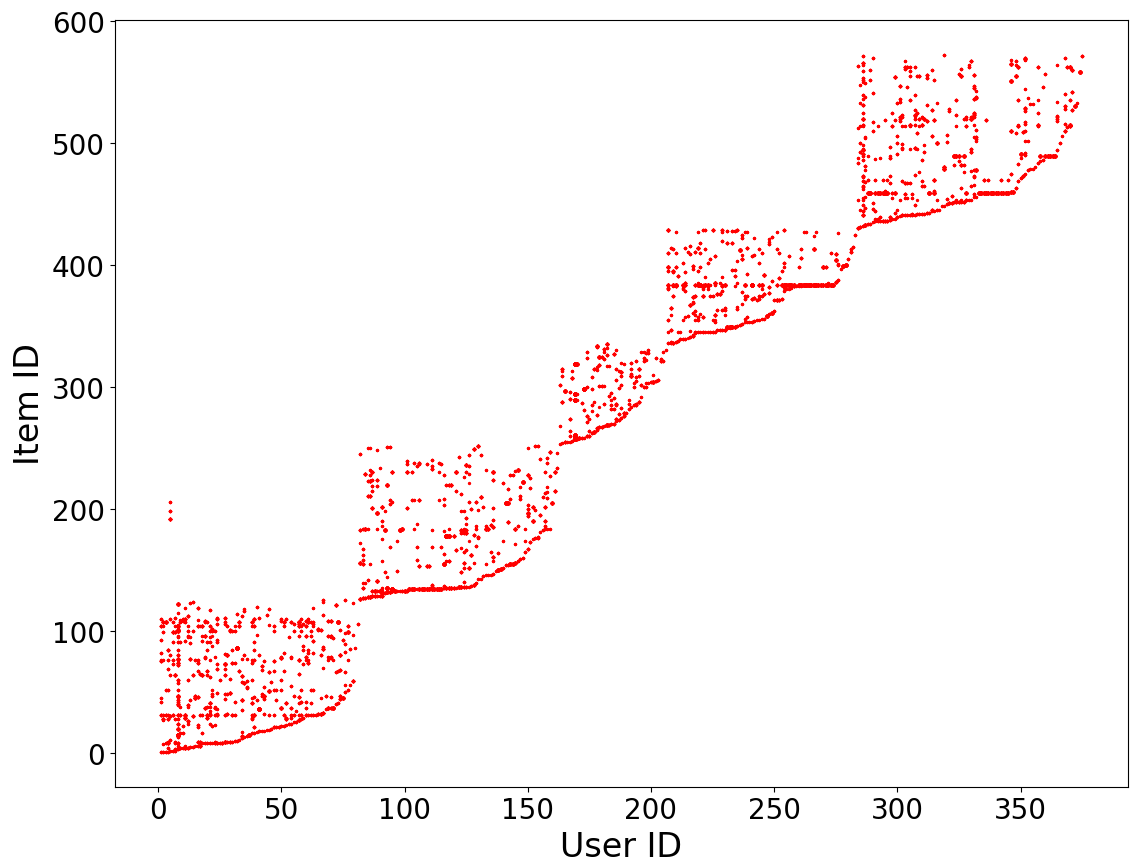
\includegraphics[width=4cm,height=3.3cm]{figures/datakb}}
%\vskip -0.15in
\caption{Data analysis of Foursquare and Alipay datasets.}
\label{dataanalysis}
%\vskip -0.15in
\end{figure}

\begin{algorithm}[t]
\caption{User communication and item latent tensor update}\label{dmfdirectneighbor}
\KwIn {current user ($i$), current item ($j$), learning rate ($\alpha$), user adjacency matrix ($W$), and item latent factor tensor ($\textbf{V}$)}
\KwOut{the updated item latent factor tensor $\textbf{V}^{new}$}
User $i$ sends $\frac{\partial \mathcal{L}}{\partial v^i_j}$ to his (directed) neighbors $i'$\\
\For{$i'$ in $\mathcal{N}(i)$}{
	Update $v^{i'}_j$ by 
	\begin{equation}\small \label{updatedelta} v^{i'}_j \leftarrow v^{i'}_j - \alpha |\mathcal{N}(i)| W_{ii'}\frac{\partial \mathcal{L}}{\partial v^i_j}\end{equation} 
}
\Return $\textbf{V}^{new}$
\end{algorithm}

\textbf{Proposal: privary preserving nearby collaboration.} 
Based on our above observation, we propose a nearby collaboration approch in decentralized POI recommendation scenarios. 
Specifically, when a user rates an item, he should send the `preference' on this item to the nearby users. 
The original rating, of course, can clearly reflect his preference on this item. 
However, the rating itself discloses the user's pravicy too much. 
Inspired by the work \cite{yan2013distributed}, we propose a privary preserving collaborative approach for decentralized POI recommendation scenarios. 
Specifically, we suppose that for each user, the corresponding $j$-th item latent factor $v^i_j$ can be decomposed as follows: 
\begin{equation}
v^i_j=h_j+h^i_j,
\end{equation} 
which implies that the latent factor of item $j$ for user $i$ is the sum between \textit{one common latent factor} $h_j$ and \textit{one personal latent factor} $h^i_j$, where the common factor represents the common preference of all the users while the personal factor shows the personal favor of user $i$. 

Gradient descent is always used to optimize MF, and the gradient with respect to item reflects a user's preference on it. 
Thus, we propose that users communicate with each other by sending their item gradients instead of raw data. 
Formally, the objective function in Equation \ref{basicdmf} becomes 
\begin{equation}\nonumber\label{comdmf}
\mathop { \min }\limits_{u_i,v^i_j \in \mathbb{R}^K} \mathcal{L} = \sum\limits_{i=1}^{I} l(r,u_i,v^i) + \frac{\lambda}{2} \sum\limits_{i=1}^I \left( ||{u_i}||_F^2 + \sum\limits_{j=1}^J||v^i_j||_F^2 \right)
\end{equation} 
\begin{equation}
{\rm s.t.} ~~ \frac{\partial \mathcal{L}}{\partial v^{i'}_j}=W_{ii'}\frac{\partial \mathcal{L}}{\partial v^i_j}, \forall ~ i' \in {\mathcal{N}(i)},
\end{equation} 
where the gradients of $\mathcal{L}$ with respect to $u_i$ and $v^i_j$ are:
\begin{equation}
\label{usergradient}
\frac{\partial \mathcal{L}}{\partial u_i} = -{\left(r_{ij} - u_i^T v^i_j\right)}v^i_j + \lambda u_{i},
\end{equation} 
\begin{equation}
\label{itemgradient}
\frac{\partial \mathcal{L}}{\partial v^i_j} = -{\left(r_{ij} - u_i^T v^i_j\right)}u_i + \lambda v^i_j.
\end{equation} 


We summarize our proposed general nearby collaborative DMF optimization framework for POI recommendation (Equation \ref{comdmf}) in Algorithm \ref{dmflearning}. 
Algorithm \ref{dmfdirectneighbor} presents how user $i$ communication with his directly neighbors and update their corresponding item latent factors. 
From it, we can see that users communicate with each other by sending their gradients instead of raw data, i.e., ratings, which significantly reduces the possibility of information leakage. 


%\textbf{Privacy discussion}. 
%Although the action of a user on an item is already a kind of pravicy no matter what is the rating ifself, which is the so-called implicit feedback in literature \cite{rendle2009bpr}, we claim the implicit feedback 
%As we can see from Algorithm \ref{dmflearning}, users communicate with each other by sending their gradients instead of raw data, i.e., ratings, which significantly reduces the possibility of information leakage. 

\textbf{Unobserved rating sample.} 
A common problem in POI recommendation is that the observations are extremely sparse. 
Unless we have access to negative observations, we will probably obtain an estimator that tends to predict all the unknow $(i,j)$ as 1 as well. 
Following the existing researches \cite{yang2011like}, we solve this problem by sampling unobserved $(i,j)$ during SGD optimization. 
Specifically, for each $r_{ij} \in \mathcal{O}$, we randomly sample $m$ missing entries $r_{ij'}, j'=1:m$ and treat them as negative examples, i.e., $r_{ij'}=0$. 
However, a missing entry $r_{ij'}$ can denote either $i$ does not like $j'$ or $i$ does not know the existing of $j'$. 
There, we decrease the confidence of $r_{ij'}$ by $1/m$. 


\subsection{Random Walk Enhanced Nearby Collaborative DMF}

\begin{figure}[!tp]
\centering
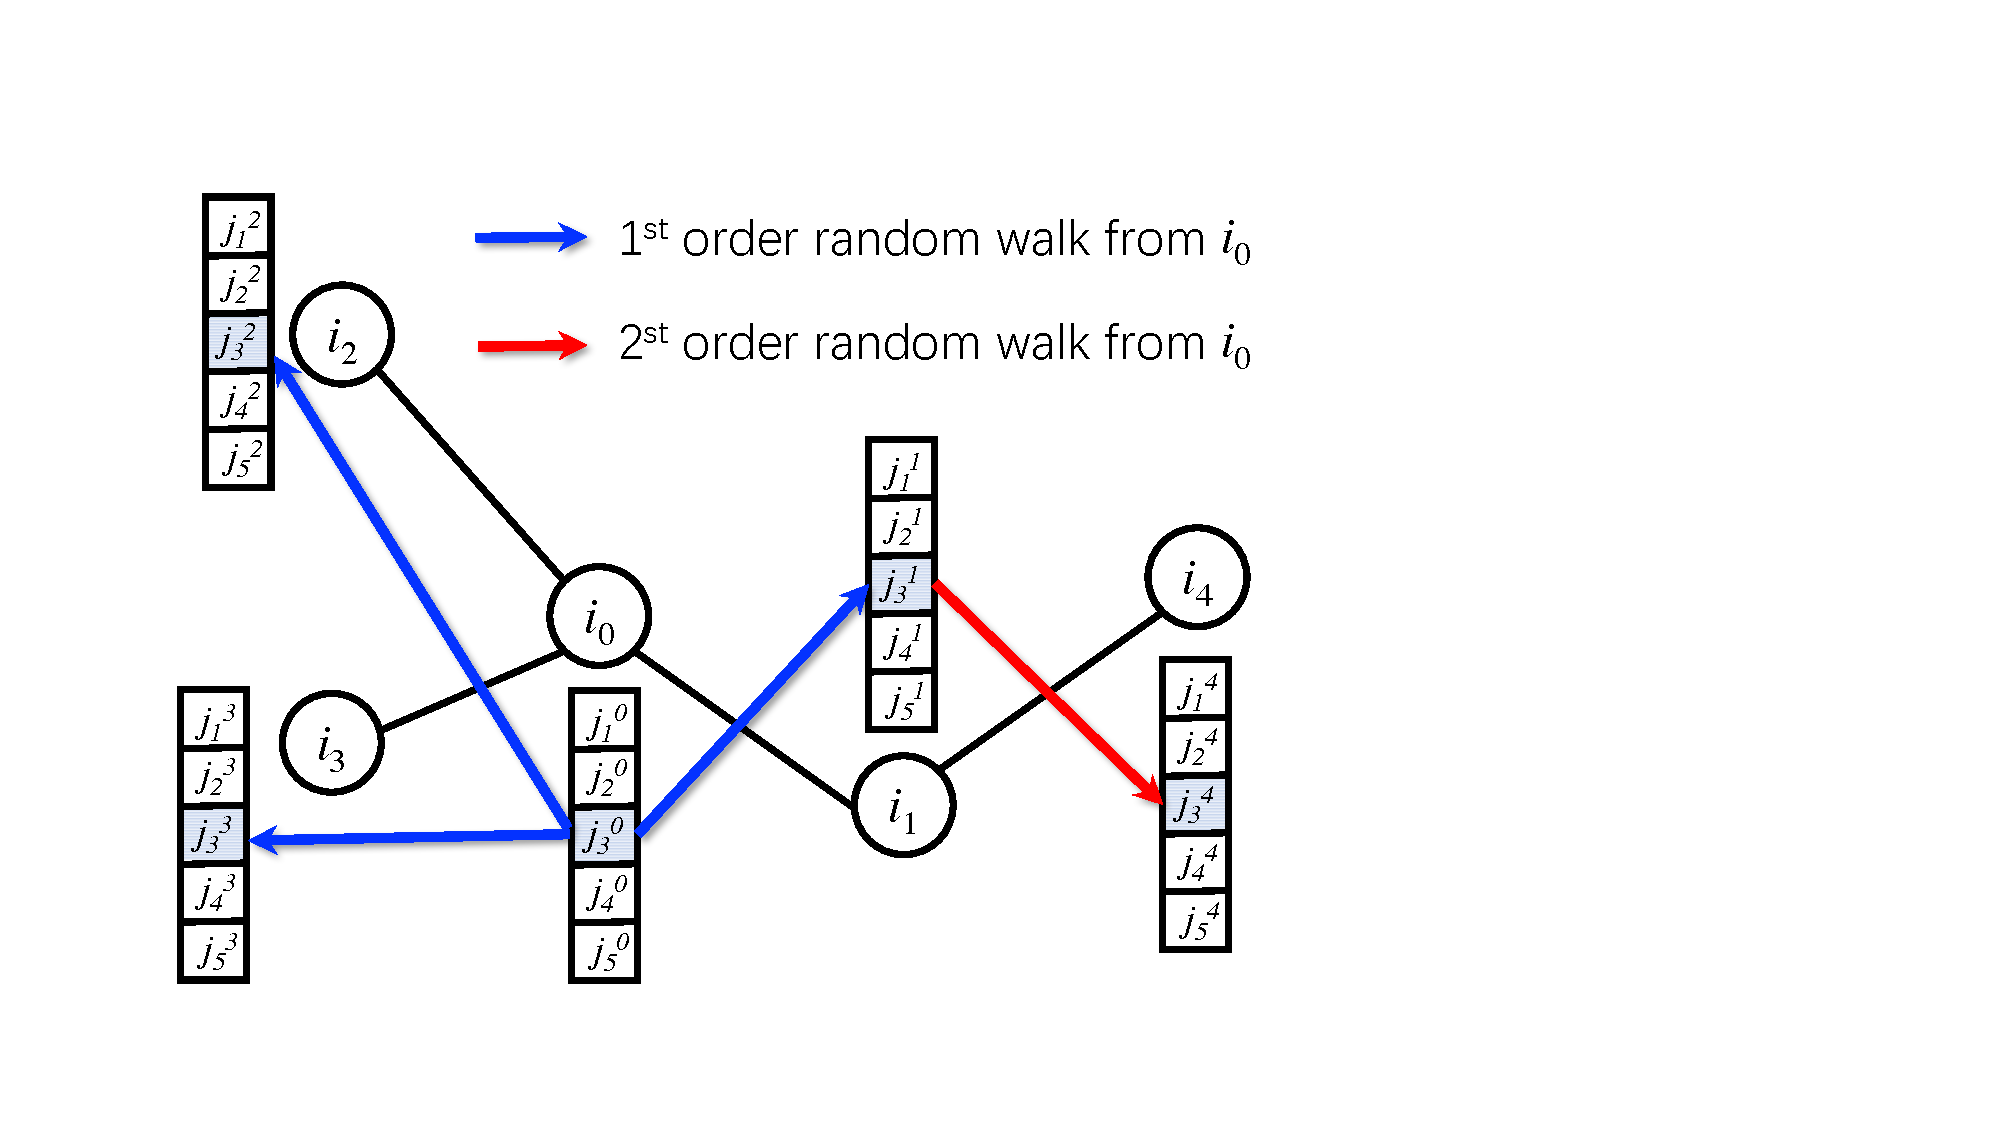
\includegraphics[width=5.5cm]{figures/randomwalk}
\vskip -0.1in
\caption{Random walk based DMF.}
\label{randomwalk}
\vskip -0.15in
\end{figure}

The adjacency matrix $W$ represents the communication graph among users, thus \textit{how far should users communication with their neighbors} becomes another challenging quesiton. 
Practically, a user's decision on an item is not only affected by his directed neighbors, but also the further neighbors, e.g., the neighbors of neighbors. 
Thus, when a user $i$ rates an item $j$, the gradient of $j$ should not only be sent to the directly neighbors of user $i$, but also his further neighbors. 
The challenge remains of how far to go in exploring the network, since there is a tradeoff between decentralization and communication/computation cost: 
the further the gradient of $j$ be sent, the more likely all the user's item latent matries tend to be the same, meanwhile, the more communication and computation need to be done. 
We propose to solve this challenge by using random walk theory. 

\textbf{Motivating example. }
Figure \ref{randomwalk} shows a motivating example of our proposed random walk enhanced DMF. 
There are 5 users and 5 items, and at a certain time, user $i_1$ rates item $j_3$. 
Then, the following things happen: 
(1) calculate the gradients of $u_1$ and $v^1_3$; 
(2) update $u_1$ and $v^1_3$ using gradient descent; 
(3) send the gradient of $v^1_3$ to the neighbors of $i_1$ using random walk strategy, which will be described in detials later; 
(4) for each $k$ in neighbors of $i_1$, update $v^k_3$ using gradient descent.

\textbf{Random walk. }
We aim to find a intelligent way to determinate how far a user send the gradients. 
Does user $i_0$ send the gradient only to his/her $1^{st}$ order of neighbors, i.e., $i_1$, $i_2$, and $i_3$, or further to his/her $2^{st}$ order of neighbors, i.e., $i_4$? 
We apply random walk to answer this question. 
Assuming user $i$ wants to send item gradient to his directed neighbors ($k \in \mathcal{N}^1(i)$), we define $n_i$ as the activity of selecting a user $k$ from $\mathcal{N}^1(i)$, and thus 
\begin{equation}
P(n_i = k) = \frac{w_{ik}}{\sum\limits_{i' \in \mathcal{N}(i)}{w_{ii'}}}. 
\end{equation} 
According to the Markov property \cite{aldous2002reversible}, the probability of user $i$ choosing his/her $2^{st}$ order of neighbors ($k' \in N(k)$) is
\begin{equation}
%P(n_i = k') \propto P(n_i = k)  P(n_k = k') = \frac{w_{ik}}{\sum\limits_{i' \in N(i)}{w_{ii'}}}  \frac{w_{kk'}}{\sum\limits_{k' \in N(k)}{w_{kk'}}}. 
P(n_i = k') = \sum\limits_{k} P(n_i = k)  P(n_k = k') \propto \sum\limits_{k} w_{ik} w_{kk'}. 
\end{equation} 
%Inspired by the work of \cite{jamali2009trustwalker}, 
We use $D$ to denote the max distance of random walk, and generally, the adjacent matrix of $d^{st}$ order of neighbors is $W^d$. 

\begin{algorithm}[t]
\caption{Random walk enhanced user communication and item latent tensor update}\label{dmfrandomwalk}
\KwIn {current user ($i$), current item ($j$), learning rate ($\alpha$), user adjacency matrix ($W$), item latent factor tensor ($\textbf{V}$), and the random walk distance ($D$)}
\KwOut{the updated item latent factor tensor $\textbf{V}^{new}$}
User $i$ sends $\frac{\partial \mathcal{L}}{\partial v^i_j}$ to his $D^{st}$ order neighbors $i'$\\
\For{$i'$ in $\sum\limits_{d=1}^D{\mathcal{N}^n(i)}$}{
	Update $v^{i'}_j$ by 
	\begin{equation}\small v^{i'}_j \leftarrow v^{i'}_j - \alpha \sum\limits_{d=1}^D{|\mathcal{N}^d(i)|} W_{ii'}\frac{\partial \mathcal{L}}{\partial v^i_j}\end{equation} 
}
\Return $\textbf{V}^{new}$
\end{algorithm}
%\vskip -0.2in

We summarize the optimization of random walk enhanced user communication and item latent tensor update procedure in Algorithm \ref{dmfrandomwalk}, and apparently, Algorithm \ref{dmfdirectneighbor} is its special case, i.e., when the random walk distance $D=1$. 
By doing this, DMF actually share only item gradient among connected users, instead of sharing the actual data. 
% Thus, comparing with the optimizing algorithm of DMF, the optimization of the $n^{st}$ order random walk enhanced DMF model has an additional input, i.e., the steps of random walk length ($N$), and Equation \ref{updatedelta} becomes 
% \begin{equation}
% v^{i'}_j \leftarrow v^{i'}_j - \alpha \sum\limits_{n=1}^N{|\mathcal{N}(i)|} W^n_{ii'}\frac{\partial \mathcal{L}}{\partial v^i_j}
% \end{equation} 


\subsection{Complexity Analysis}
Here we analyze the communication and computation complexity of the proposed random walk enhanced nearby collaborative DMF framework. 
Recall that $K$ denotes the dimension of latent factor, $N$ denotes the maximum number of directed neighbors of each user, $D$ denotes the max distance of random walk, $\mathcal{O}$ as the training data, and $|\mathcal{O}|$ as the training data size. 

\textbf{Communication Complexity. }
The communication cost depends on both the legnth of item gradient and number of neighbor to be communicated. 
Each item gradient contains $K \cdot 4b$ information, since it is a $K$ dimensional real valued vector. 
The max number of neighbor of $D^{st}$ order random walk is $N^D$. 
Thus, for each $r_{ij} \in \mathcal{O}$, the communication cost is $N^D \cdot K \cdot 4b$. 
It will be $|\mathcal{O}| \cdot N^D \cdot K \cdot 4b$ for passing the training dataset once. 
The values of $N$, $D$, and $K$ are usually small, and thus the communication cost is linear with the training data size. 

\textbf{Computation Complexity. }
The computation cost mainly relies on two parts, (1) calculating user and item gradients, i.e., Line 7 in Algorithm \ref{comdmf}, and (2) updating user and item latent factors, i.e., Line 8 in Algorithm \ref{comdmf}. 
For a single pass of the training data, the time complexity of (1) is $|\mathcal{O}| \cdot K$, and the time complexity of (2) is $|\mathcal{O}| \cdot N^D \cdot K$. 
Therefore, the total computational complexity in one iteration is $|\mathcal{O}| \cdot N^D \cdot K$. 
Also, the values of $N$, $D$, and $K$ are usually small, and thus the time complexity is linear with the training data size. 

The above communication and computation complexity analysis shows that our proposed approach is very efficient and can scale to very large datasets. 

%\subsection{Generalization}
%Our proposed decentralized MF framework has good extensibility, which can be easily modified to adapt to scenarios where other kinds of information are available. For example, when social or contextual information ...